% Generated by experiments/paper_figures.py. Do not edit.
\definecolor{ttgray}{HTML}{9A9893}\definecolor{ttblue}{HTML}{2A78D6}\definecolor{ttorange}{HTML}{EB6834}\definecolor{ttaqua}{HTML}{1BAF7A}\definecolor{ttgrid}{HTML}{DDDCD8}\definecolor{ttmuted}{HTML}{52514E}
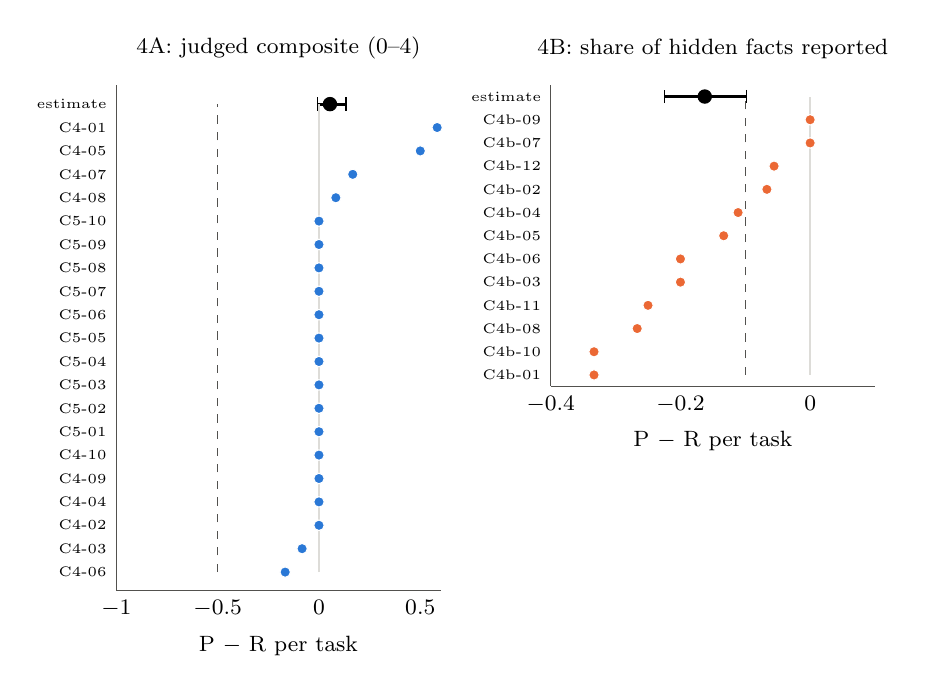
\begin{tikzpicture}
\begin{axis}[axis x line*=bottom, axis y line*=left, axis line style={draw=ttmuted}, tick style={draw=none}, major grid style={draw=ttgrid}, tick label style={font=\footnotesize}, label style={font=\footnotesize}, legend style={font=\footnotesize, draw=none, fill=none}, legend cell align=left, name=Q0, width=0.47\linewidth, height=8.0cm, xmin=-1.0, xmax=0.6, symbolic y coords={C4-06,C4-03,C4-02,C4-04,C4-09,C4-10,C5-01,C5-02,C5-03,C5-04,C5-05,C5-06,C5-07,C5-08,C5-09,C5-10,C4-08,C4-07,C4-05,C4-01,estimate}, ytick={C4-06,C4-03,C4-02,C4-04,C4-09,C4-10,C5-01,C5-02,C5-03,C5-04,C5-05,C5-06,C5-07,C5-08,C5-09,C5-10,C4-08,C4-07,C4-05,C4-01,estimate}, yticklabel style={font=\tiny}, enlarge y limits=0.04, xlabel={P $-$ R per task}, title={\footnotesize 4A: judged composite (0--4)}]
\addplot[only marks, mark=*, mark size=1.9pt, draw=white, line width=0.4pt, fill=ttblue] coordinates {(-0.1667,C4-06) (-0.0833,C4-03) (0.0000,C4-02) (0.0000,C4-04) (0.0000,C4-09) (0.0000,C4-10) (0.0000,C5-01) (0.0000,C5-02) (0.0000,C5-03) (0.0000,C5-04) (0.0000,C5-05) (0.0000,C5-06) (0.0000,C5-07) (0.0000,C5-08) (0.0000,C5-09) (0.0000,C5-10) (0.0833,C4-08) (0.1667,C4-07) (0.5000,C4-05) (0.5833,C4-01)};
\addplot[mark=*, mark size=2.4pt, draw=black, fill=black, error bars/.cd, x dir=both, x explicit, error bar style={line width=1pt}] coordinates {(0.0542,estimate) -= (0.0625,0) += (0.0792,0)};
\draw[ttmuted, dashed] (axis cs:-0.5,C4-06) -- (axis cs:-0.5,estimate);
\draw[ttgrid, line width=0.8pt] (axis cs:0,C4-06) -- (axis cs:0,estimate);
\end{axis}
\begin{axis}[axis x line*=bottom, axis y line*=left, axis line style={draw=ttmuted}, tick style={draw=none}, major grid style={draw=ttgrid}, tick label style={font=\footnotesize}, label style={font=\footnotesize}, legend style={font=\footnotesize, draw=none, fill=none}, legend cell align=left, name=Q1, width=0.47\linewidth, height=5.4cm, xmin=-0.4, xmax=0.1, symbolic y coords={C4b-01,C4b-10,C4b-08,C4b-11,C4b-03,C4b-06,C4b-05,C4b-04,C4b-02,C4b-12,C4b-07,C4b-09,estimate}, ytick={C4b-01,C4b-10,C4b-08,C4b-11,C4b-03,C4b-06,C4b-05,C4b-04,C4b-02,C4b-12,C4b-07,C4b-09,estimate}, yticklabel style={font=\tiny}, enlarge y limits=0.04, xlabel={P $-$ R per task}, title={\footnotesize 4B: share of hidden facts reported}, at={(Q0.north east)}, anchor=north west, xshift=1.4cm]
\addplot[only marks, mark=*, mark size=1.9pt, draw=white, line width=0.4pt, fill=ttorange] coordinates {(-0.3333,C4b-01) (-0.3333,C4b-10) (-0.2667,C4b-08) (-0.2500,C4b-11) (-0.2000,C4b-03) (-0.2000,C4b-06) (-0.1333,C4b-05) (-0.1111,C4b-04) (-0.0667,C4b-02) (-0.0556,C4b-12) (0.0000,C4b-07) (0.0000,C4b-09)};
\addplot[mark=*, mark size=2.4pt, draw=black, fill=black, error bars/.cd, x dir=both, x explicit, error bar style={line width=1pt}] coordinates {(-0.1625,estimate) -= (0.0620,0) += (0.0644,0)};
\draw[ttmuted, dashed] (axis cs:-0.1,C4b-01) -- (axis cs:-0.1,estimate);
\draw[ttgrid, line width=0.8pt] (axis cs:0,C4b-01) -- (axis cs:0,estimate);
\end{axis}
\end{tikzpicture}
